\section{Results} \label{sec:results}


\subsection{PTC}

As part of this project, a key initial task was to utilize the PTC to determine essential parameters for each CCD segment across the focal plane using the \textit{DM stack}. This has already been done by SLAC National Accelerator Laboratory\footnote{The code used by SLAC is available at \href{https://github.com/lsst-camera-dh/eotest/blob/32c17b0a33b9c099651ed581ee90c1b1101012fb/python/lsst/eotest/sensor/ptcTask.py}{SLAC code}} (referred to as SLAC hereafter) for this particular run (\href{https://srs.slac.stanford.edu/BOT_EO_Reports/13144/}{SLAC heat maps BOT 13144}), and we aim to reproduce their results in this study.

\vspace{3mm}

%%%%%%%%%%%%Figura

\begin{figure}[!htb]
    \centering
    \includegraphics[width=\textwidth]{Figures/PTC_Detector55.png}
    \caption{PTC for all segments of sensor 55 (E2V). The Xs represent the data points, the red line is the exponential fit to the PTC using the Astier16 approximation (eq. \ref{eq:Astier16}), and the green line is a linear fit. The obtained fit parameters include the gain, the $a_{00}$ parameter, the PTC turnoff (Max ADU), and the read noise.}
    \label{fig:PTC_55}
\end{figure}

%%%%%%%%%%%%%%%%%%

Initially, PTCs were generated by CCD for the entire focal plane, as shown in Figure \ref{fig:PTC_55}, to detect any abnormal behavior and low PTC-turnoff values (below 40000 ADU). Detectors found with low PTC-turnoff and/or misclassified were recorded in Table \ref{tab:PTC_warnings}. Furthermore, a visual inspection revealed that approximately 60 \% of the detectors had at least one segment exhibiting a \textit{Downing dip}.

\vspace{3mm}
%%%%%%%%%%%%Figura

\begin{figure}[!htb]
 \centering
     \begin{subfigure}[b]{0.49\textwidth}
         \centering
         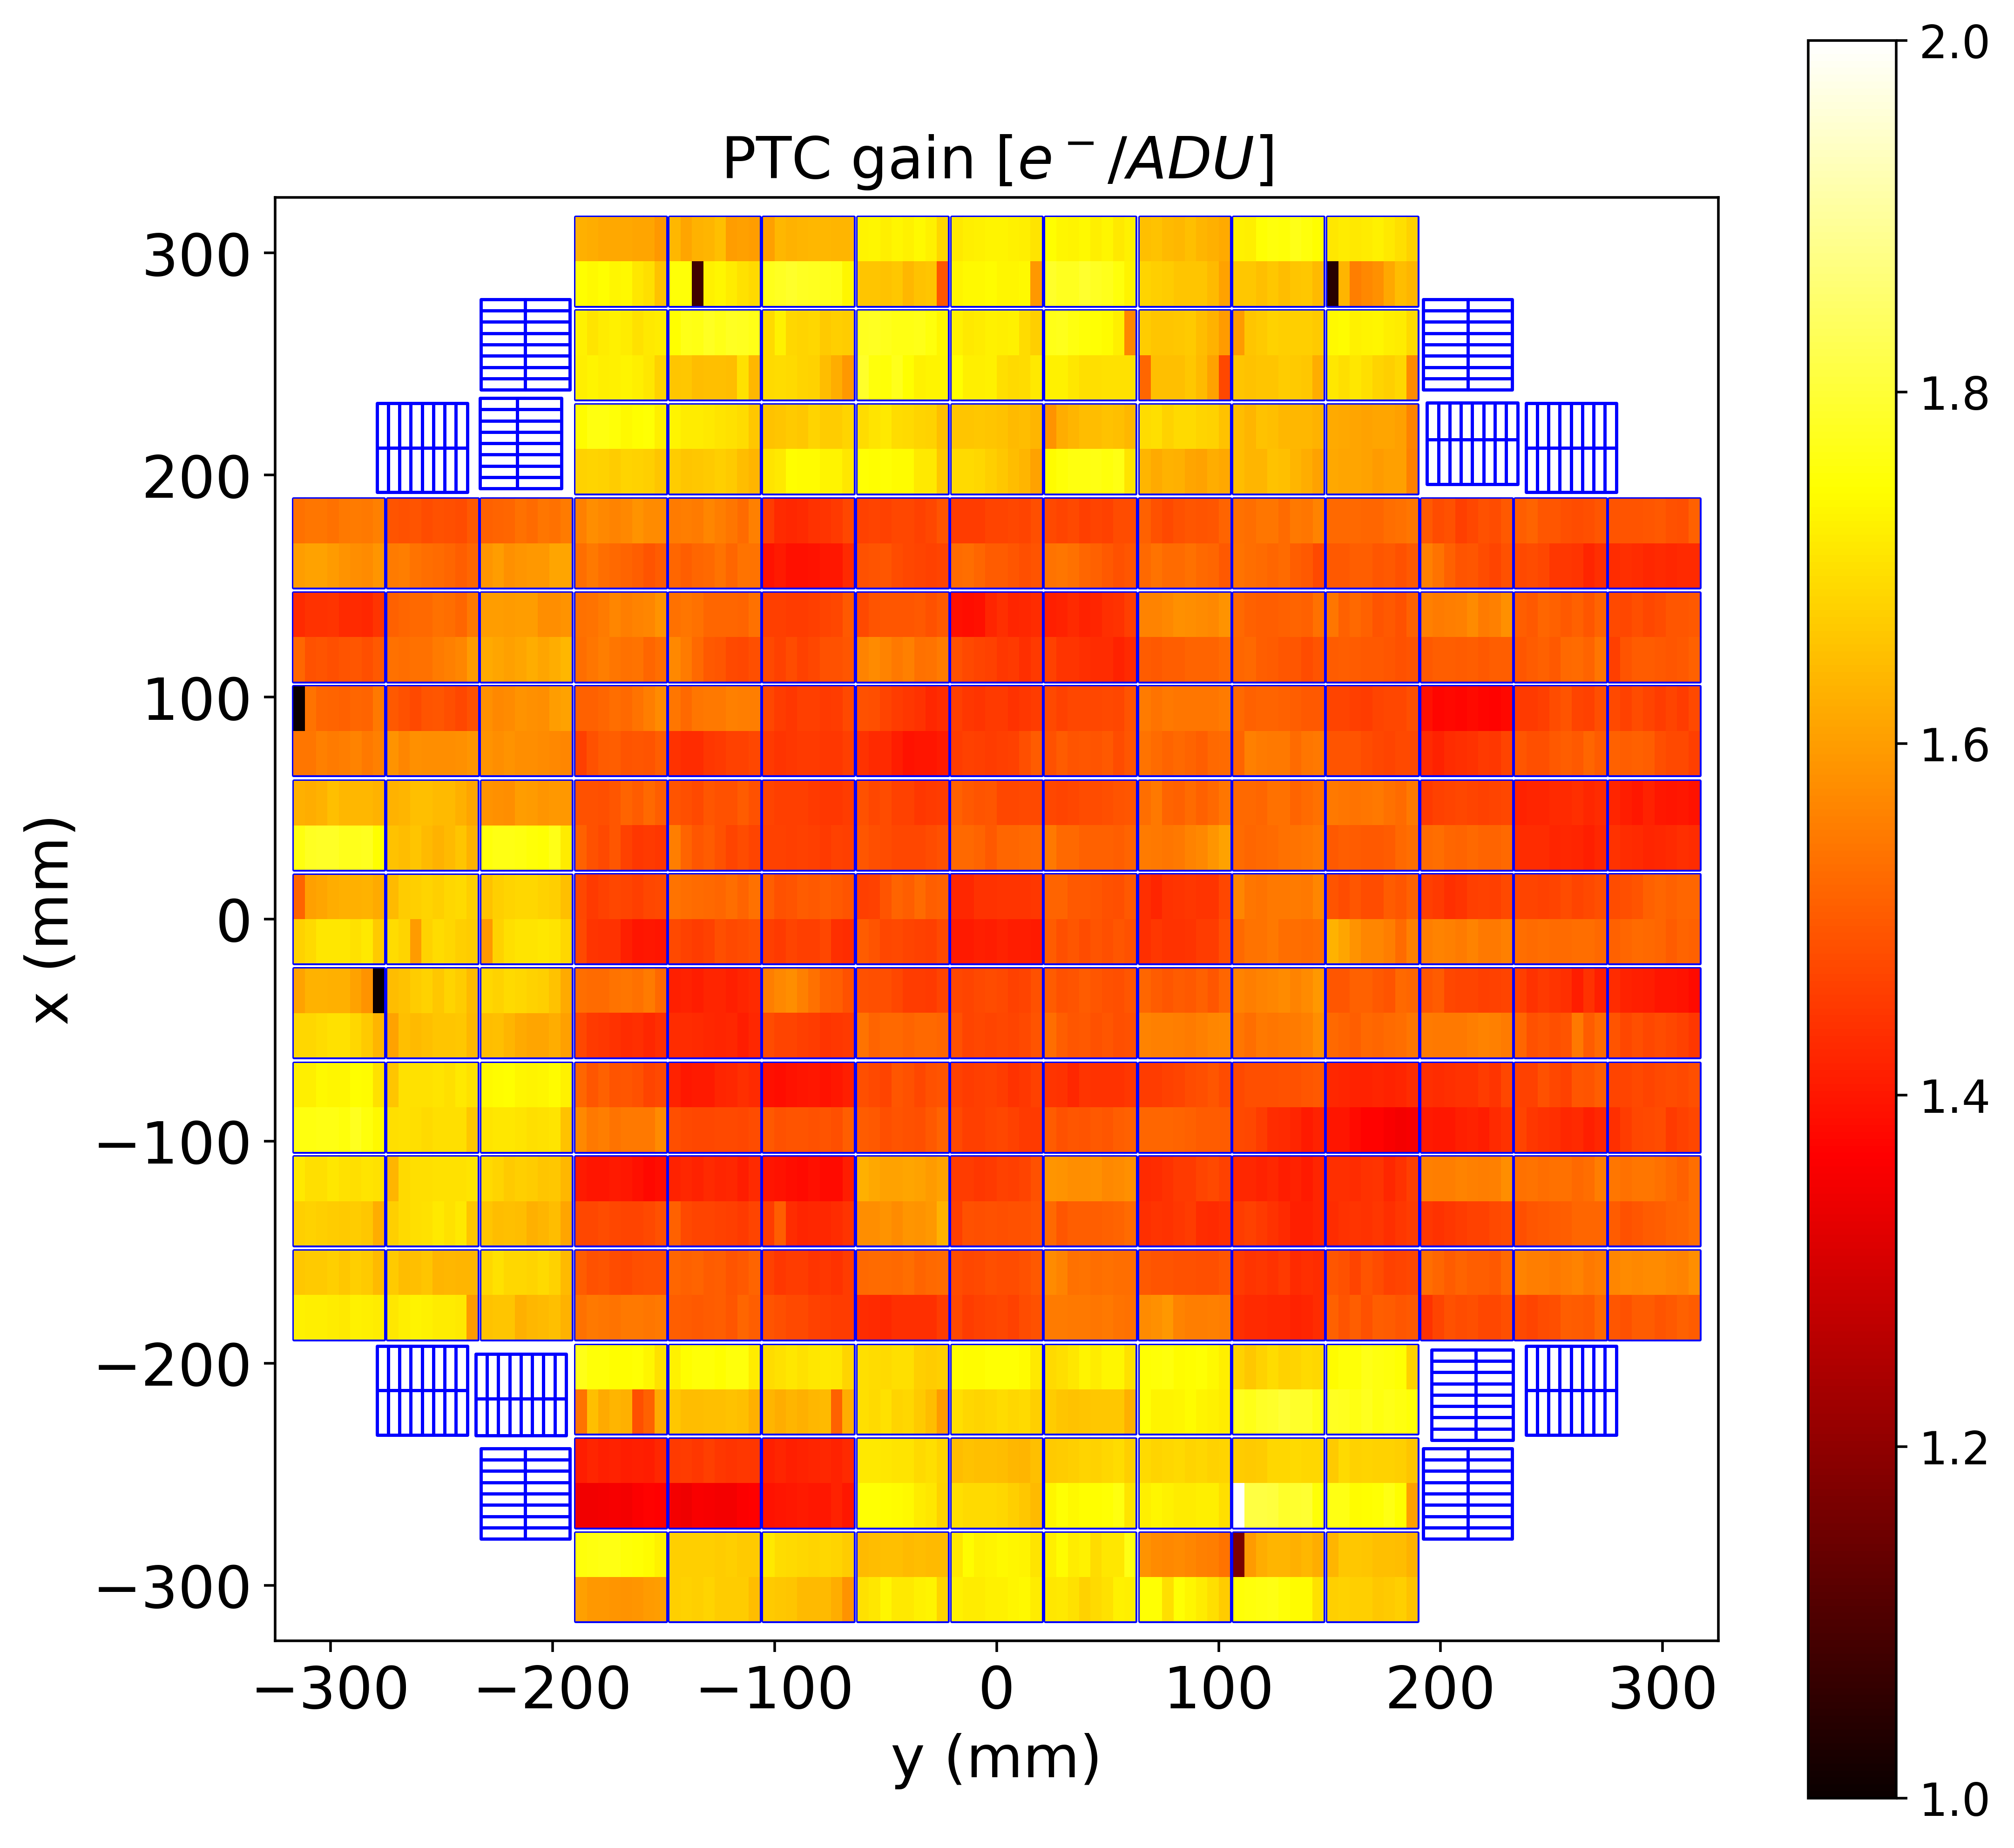
\includegraphics[width=\textwidth]{Figures/Focal_plane_gain.png}
     \end{subfigure}
     \hfill %\hspace{-10em}
     \begin{subfigure}[b]{0.49\textwidth}
         \centering
         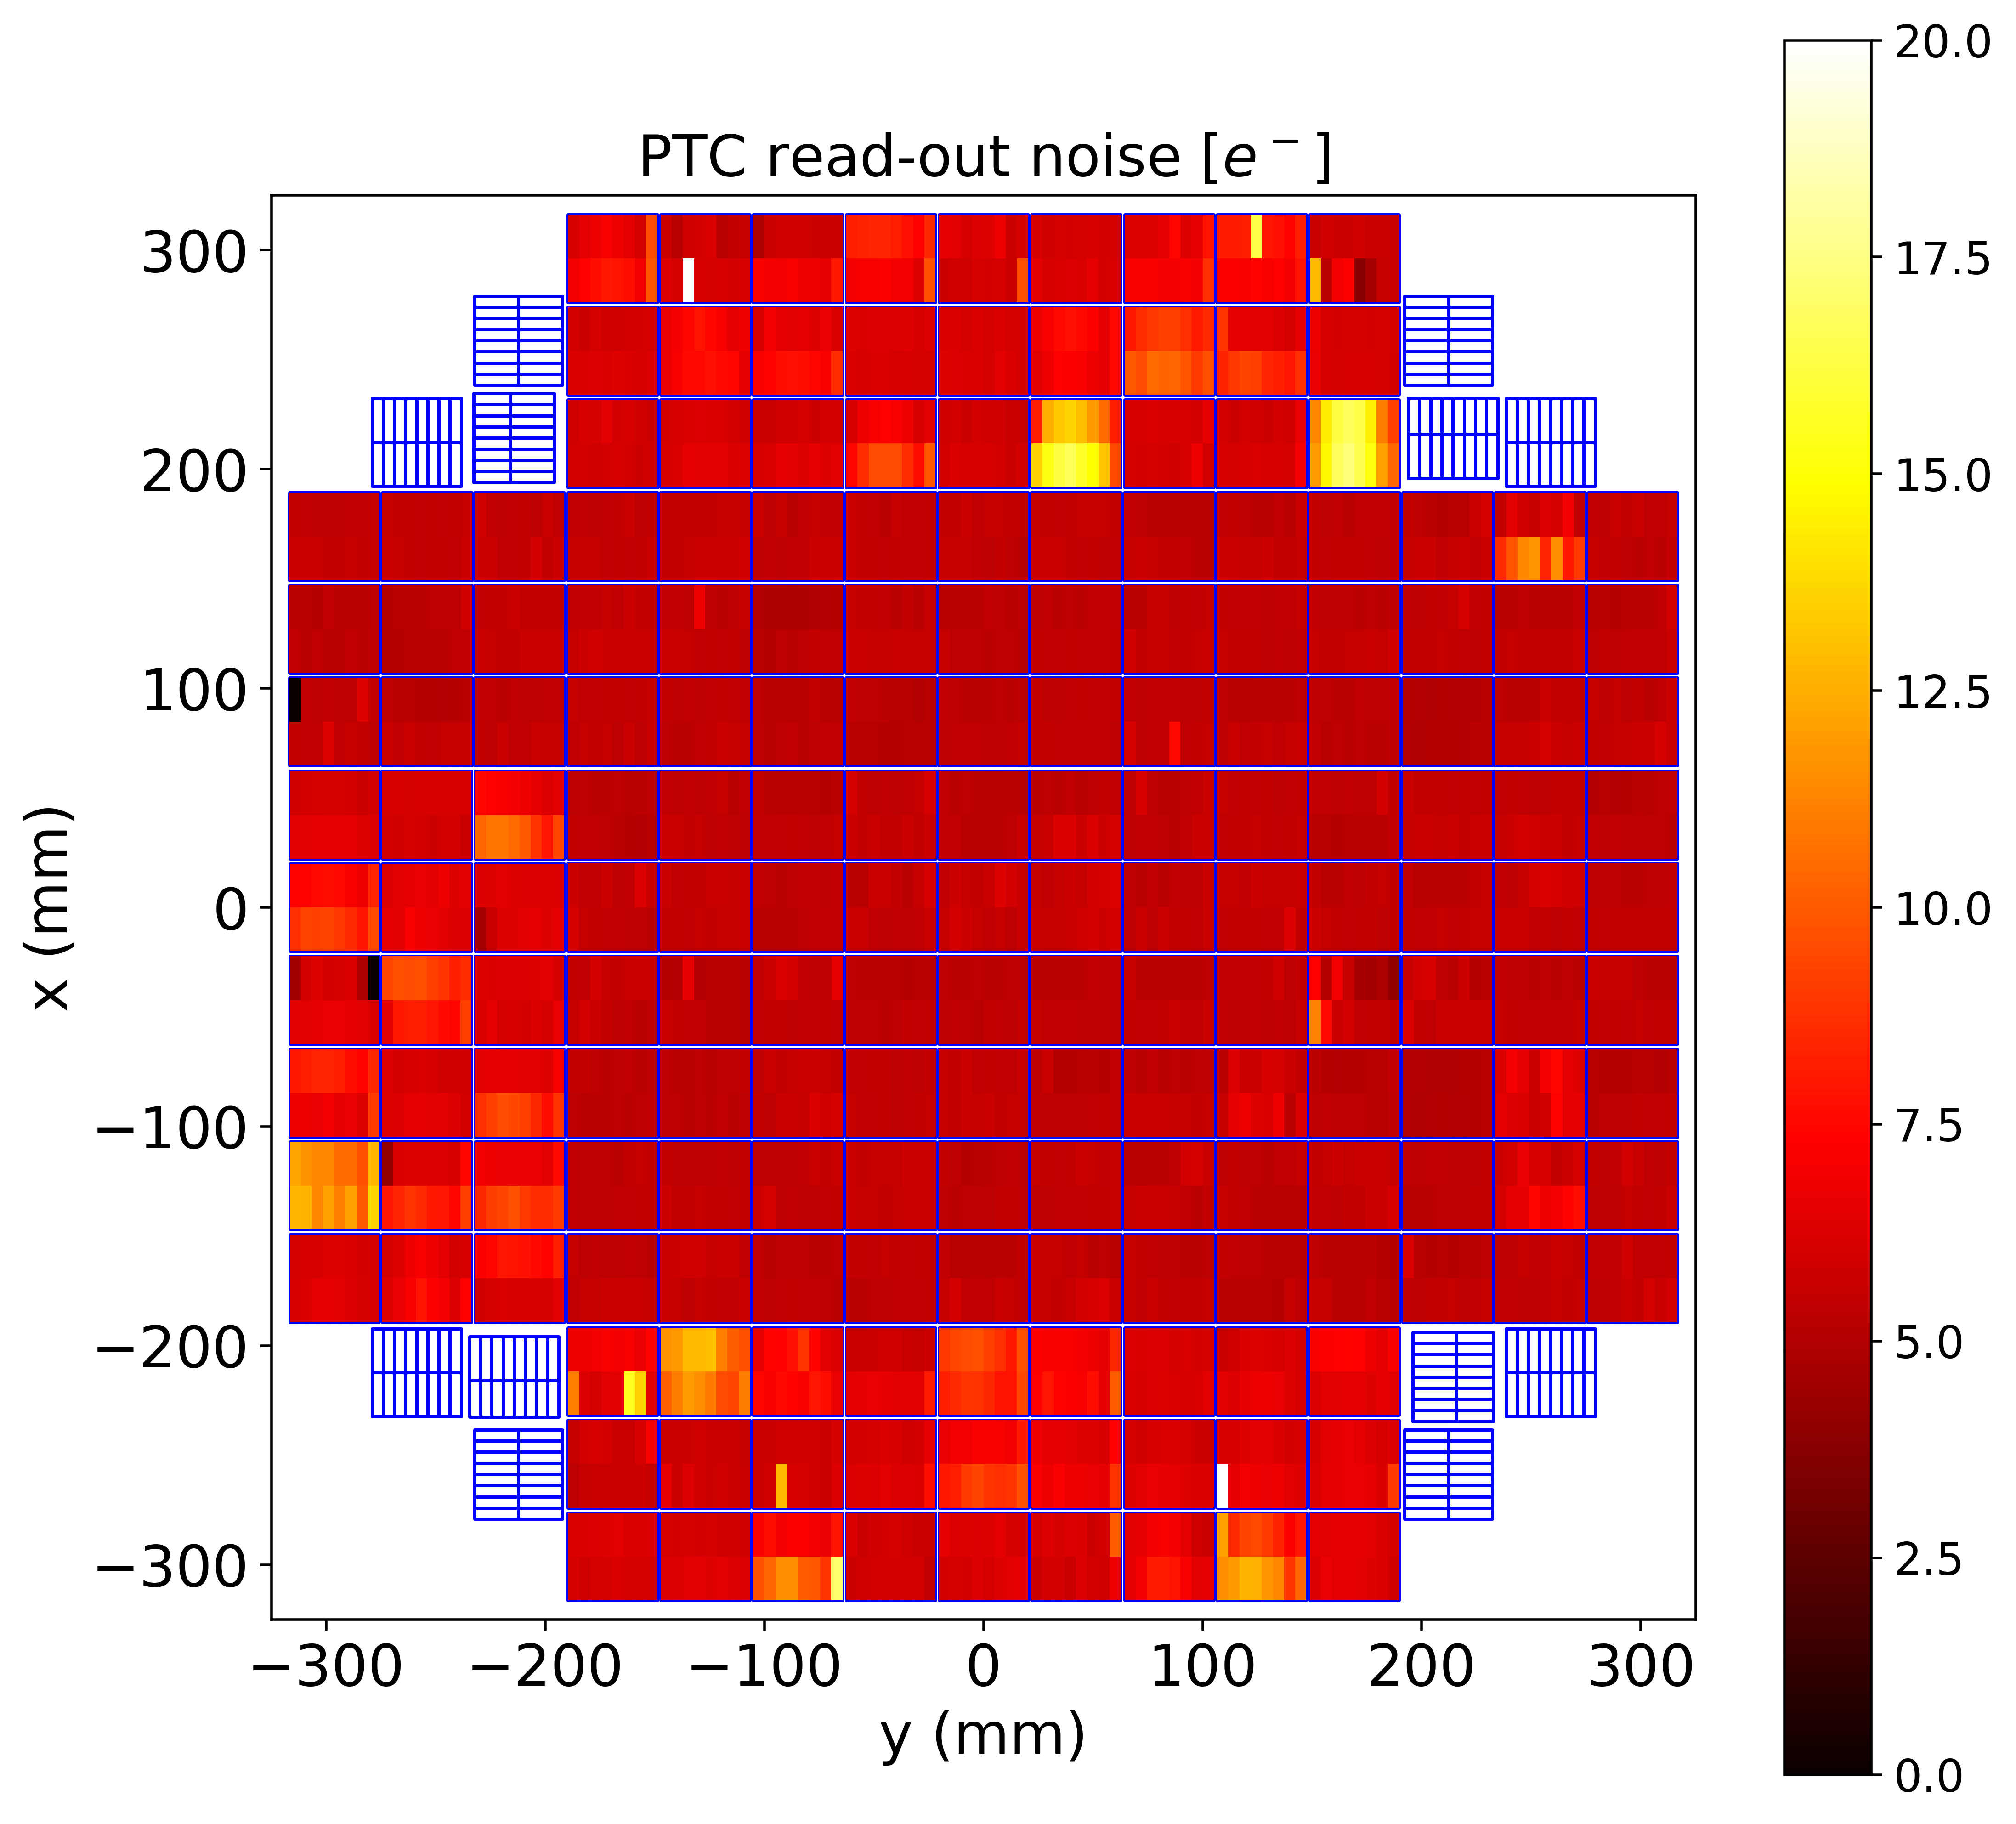
\includegraphics[width=\textwidth]{Figures/Focal_plane_noise.png}
     \end{subfigure}
     \vspace{3mm}
     \begin{subfigure}[b]{0.49\textwidth}
         \centering
         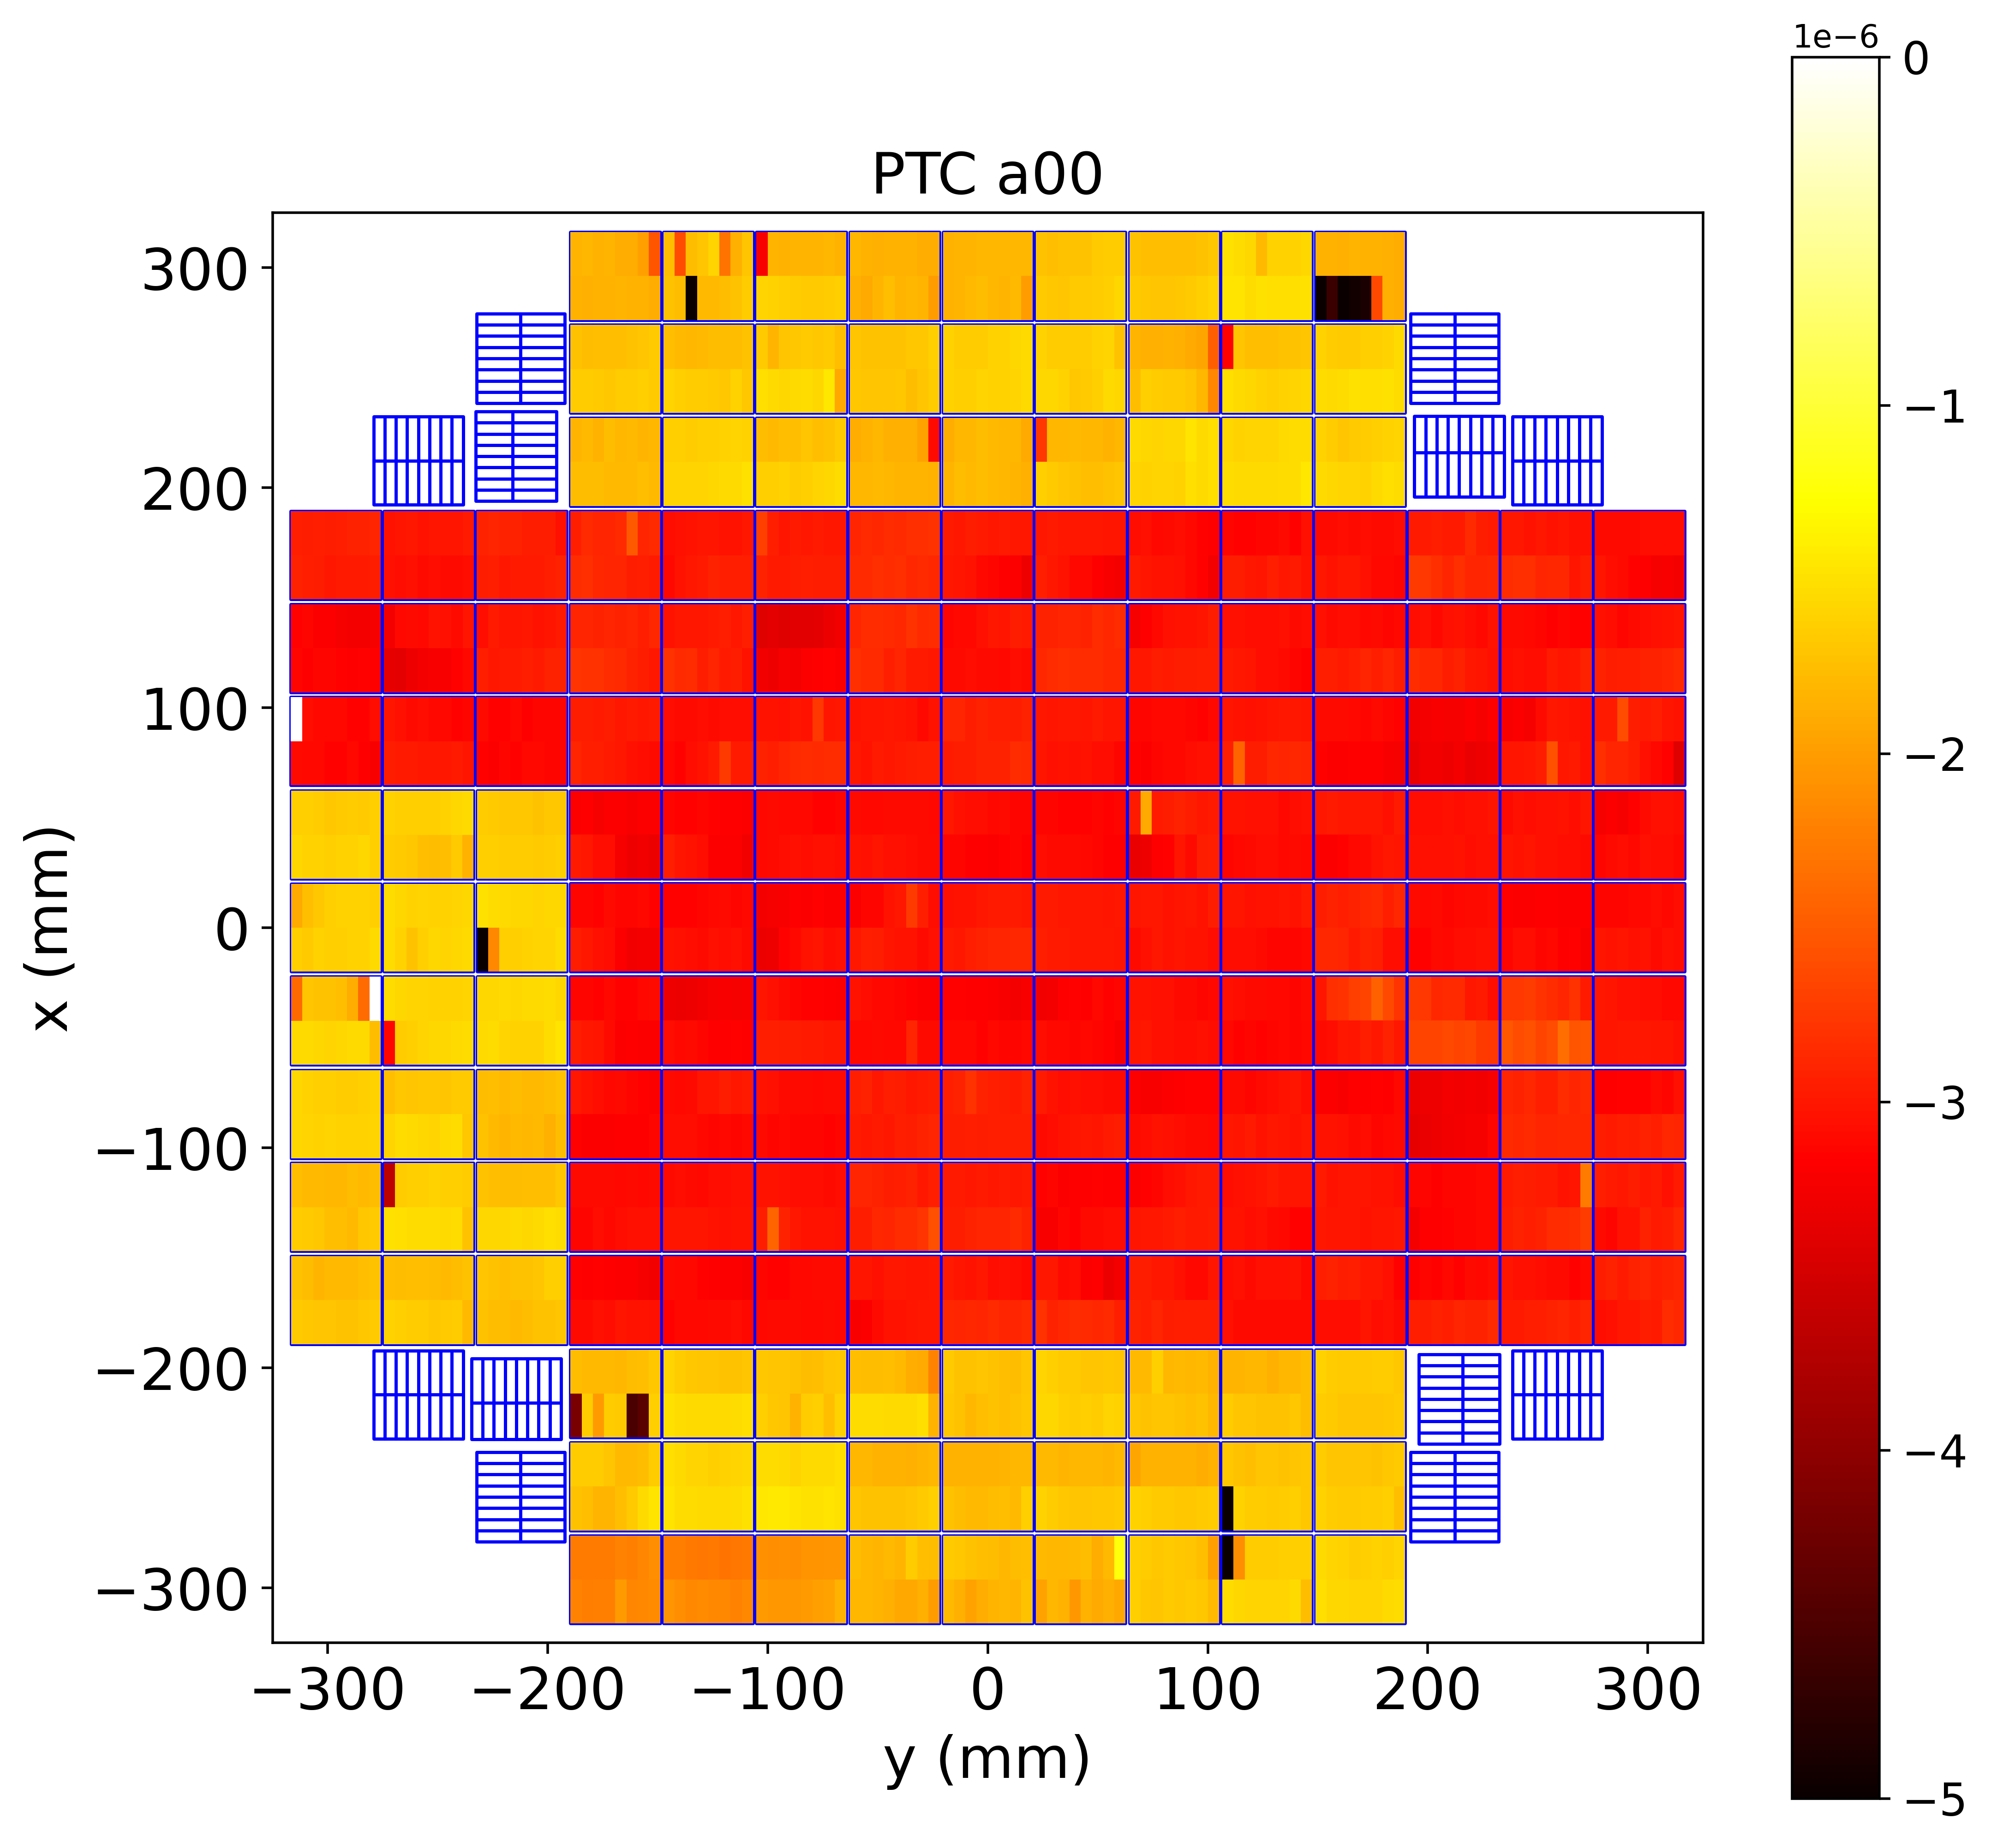
\includegraphics[width=\textwidth]{Figures/Focal_plane_a00.png}
     \end{subfigure}    
     \hfill
     \begin{subfigure}[b]{0.49\textwidth}
         \centering
         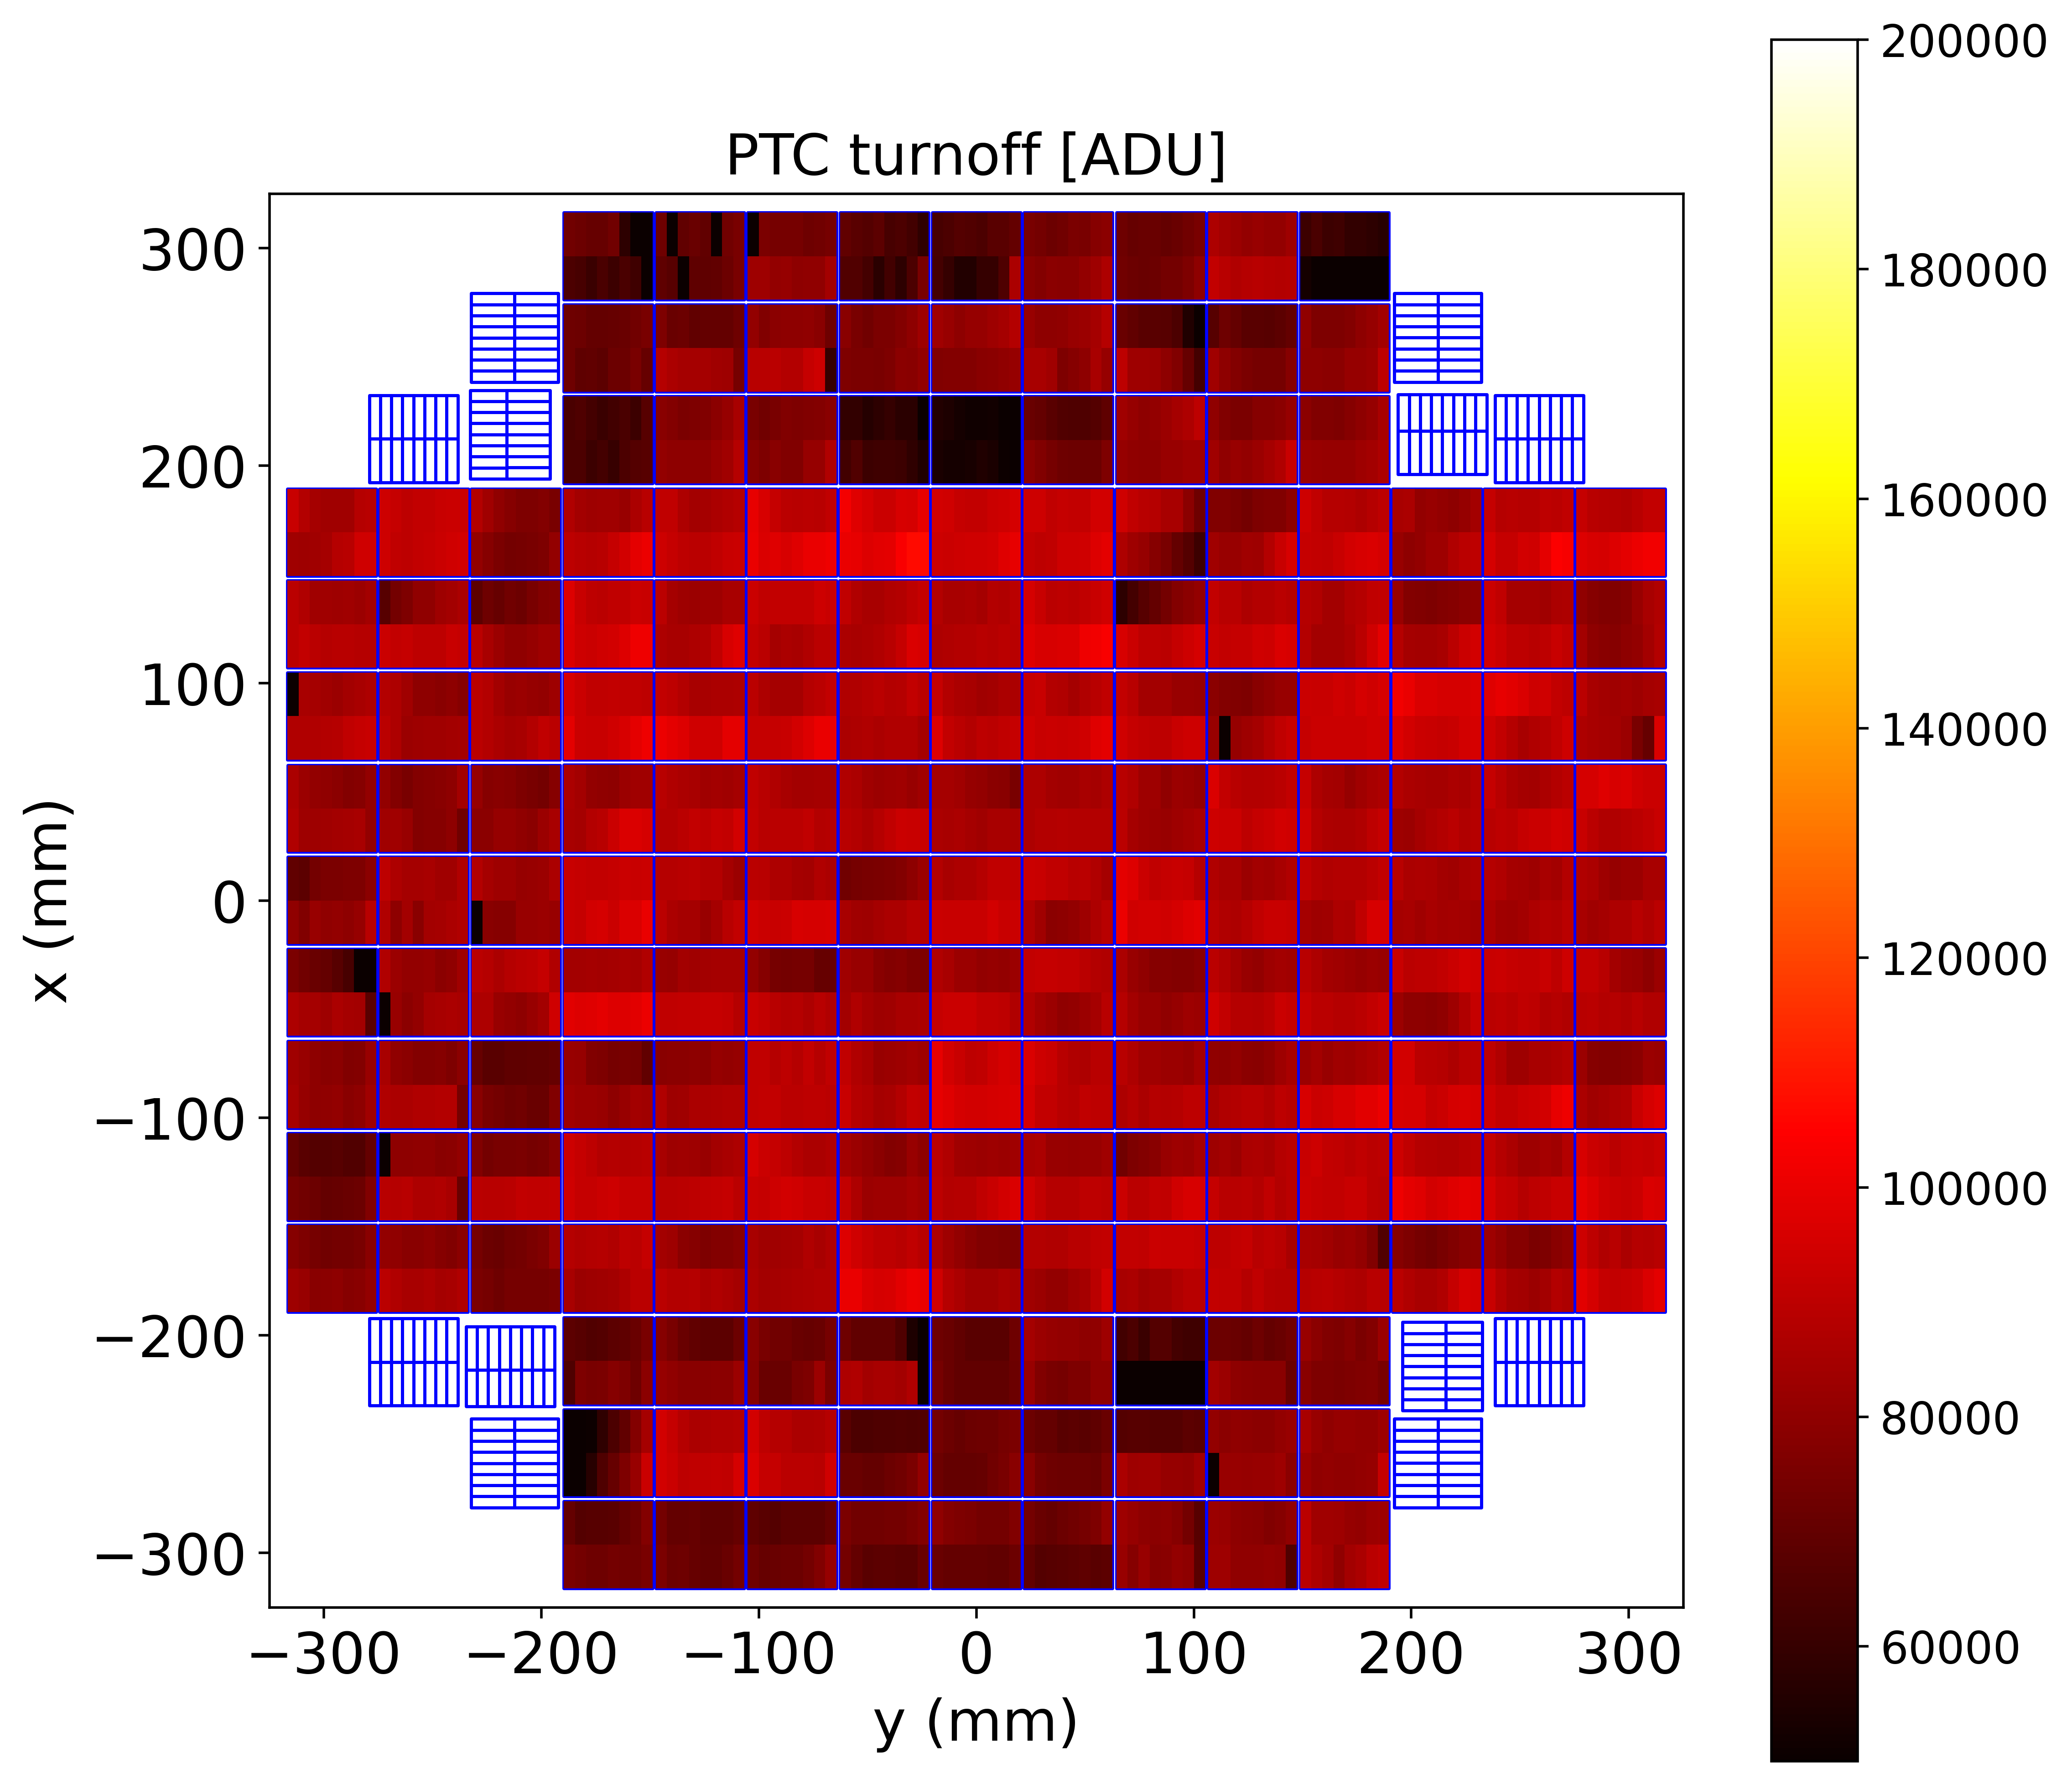
\includegraphics[width=\textwidth]{Figures/Focal_plane_turnoff.png}
     \end{subfigure}
        \caption{Heatmaps depicting the parameters obtained by fitting the PTC for each segment of the sensors across the entire focal plane. The upper panel shows the gain values on the left and the read noise on the right. The lower panel shows the values of $a_{00}$, which are of the order of $-1 \times 10 ^{-6}$, on the left, and the turnoff on the right. These maps are a reproduction of those previously constructed by SLAC for the same run 13144 (\href{https://srs.slac.stanford.edu/BOT_EO_Reports/13144/}{SLAC heat maps}.}
        \label{fig:FocalPlane_PTC}
\end{figure}
%%%%%%%%%%%%%%%%%%
Subsequently, heat maps were generated for the entire focal plane, similar to those performed by SLAC, as shown in the panels of Figure \ref{fig:FocalPlane_PTC}, to visualize the parameters estimated by fitting the PTC: gain and read noise in the upper left and right panels, respectively, and $a_{00}$ and turnoff in the lower left and right panels, respectively. Notably, bimodality is observed in the gain and $a_{00}$ values, which account for the BF effect. The more reddish values dominate in the E2V sensors, while the more yellow values dominate in ITL sensors, indicating that E2V vendor's detectors generally have a lower gain but more negative BF effect coefficients compared to ITL. In contrast, no significant effect is exhibited due to the vendor for readout noise and turnoff.

\vspace{3mm}
The histograms in Figure \ref{fig:Histogram_PTC} support the behavior described above by the heat maps, revealing clear bimodality for gain and $a_{00}$, and a more generalized behavior for read noise and turnoff. The average gain values for E2V sensors are $1.49 \pm 0.05$ $e^{-}/ADU$, and for ITL sensors are $1.69 \pm 0.05$ $e^{-}/ADU$. The average BF effect coefficient values are $(-3.0 \pm 0.1)\times 10 ^{-6}$ for E2V and $(-1.7 \pm 0.2)\times 10 ^{-6}$ for ITL.

\vspace{3mm}

%%%%%%%%%%%%Figura
\begin{figure}[!htb]
    \centering
    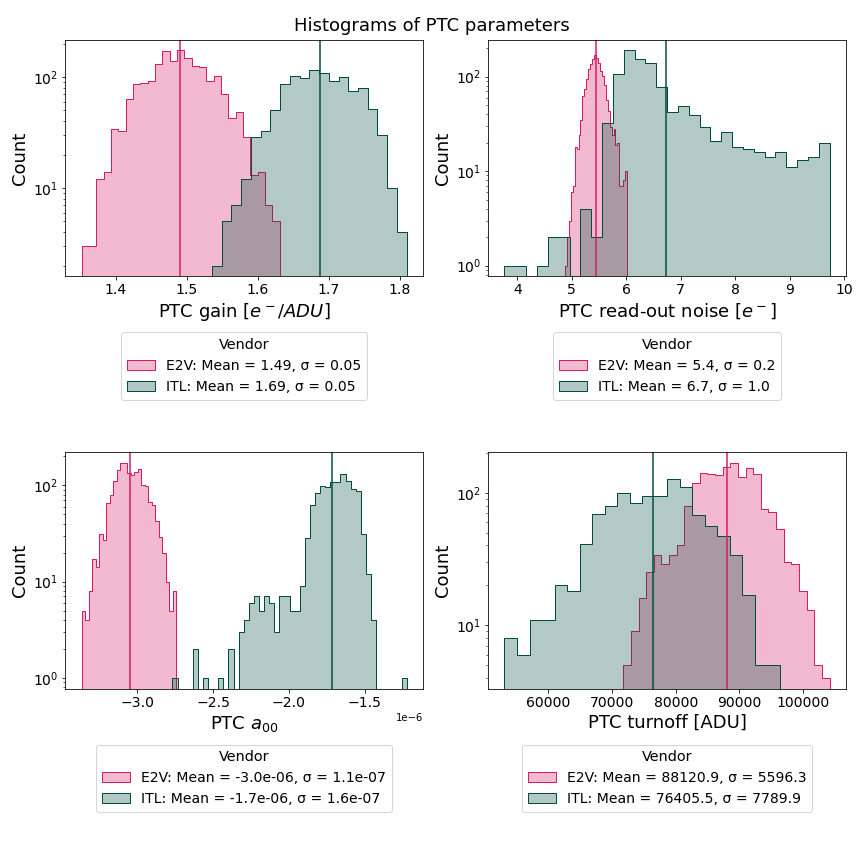
\includegraphics[width=\textwidth]{Figures/Histograms_PTC.png}
    \caption{Histograms showing the distribution of parameters obtained from the fit to the PTC: gain (top left), read noise (top right), $a_{00}$ (bottom left), and turnoff (bottom right). The distributions are shown separately for each vendor, with magenta representing E2V and blue representing ITL. The vertical lines indicate the mean value of each distribution.}
    \label{fig:Histogram_PTC}
\end{figure}

%%%%%%%%%%%%%%%%%%
Although the results of this work are generally congruent with those obtained by SLAC, some differences were found in certain segments, particularly for gain values in segments C04 and C14 of detector 0 (R01\_S00), C00 of detector 22 (R03\_S11), and C02 of detector 169 (R41\_S21). Table \ref{tab:PTC_warnings} highlights these segments in red, where the most notable differences between our results and those of SLAC were observed for the four parameters (gain, BF coefficient, read noise, and turnoff). For detector 22, the values on the table suggest that the detector may possibly be dead, while for the segment of detector 169, there may be a misclassification by the PTC-turnoff location algorithm. These specific cases could be the reason for the differences between our results and those of SLAC. However, to determine the precise cause of these differences, a detailed analysis of the respective codes used and their versions is necessary. Discrepancies between the algorithms could arise from various factors, such as differences in the pixels used for calculation due to masks applied, variations in the image reduction techniques (e.g., Instrument Signature Removal or ISR), or differences in the rejection of outliers, among others. Further investigation is needed to elucidate the exact source of these discrepancies as we utilized the same run (13144) as SLAC.

\vspace{3mm}

%%%%%%%%%%%%Figura

\begin{figure}[!htb]
%\raggedleft
     \begin{subfigure}[b]{\textwidth}
         
         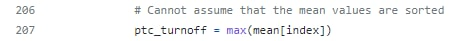
\includegraphics[width=0.7\textwidth,left]{Figures/eotest_turnoff.jpg}
         \caption{Eotest code}
     \end{subfigure}
     \vspace{3mm}
     \begin{subfigure}[b]{\textwidth}
         
         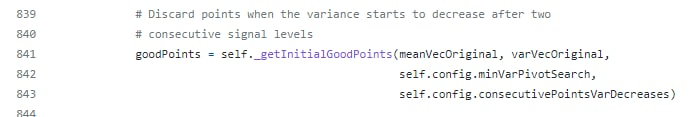
\includegraphics[width=\textwidth,left]{Figures/DMstack_turnoff1.jpg}
     \end{subfigure}    
     \vspace{3mm}
     \begin{subfigure}[b]{\textwidth}
         
         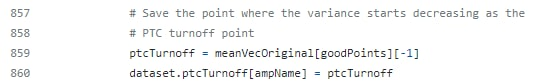
\includegraphics[width=0.85\textwidth,left]{Figures/DMstack_turnoff2.jpg}
         \caption{DM stack code}
     \end{subfigure}
        \caption{Codes used to calculate the PTC-turnoff in \href{https://github.com/lsst-camera-dh/eotest/blob/32c17b0a33b9c099651ed581ee90c1b1101012fb/python/lsst/eotest/sensor/ptcTask.py}{eotest} (a), employed by SLAC, and \href{https://github.com/lsst/cp_pipe/blob/6bae47012f2f119b186509ce7efd963b68b61f0d/python/lsst/cp/pipe/ptc/cpSolvePtcTask.py}{DM stack} (b), the official code for LSST data.}
        \label{fig:Turnoff_codes}
\end{figure}
%%%%%%%%%%%%%%%%%%
Overall, we observed similar behavior for the turn-off of the sensors between our work and SLAC, although the methods used for determination were different, as shown in Figure \ref{fig:Turnoff_codes}. In \textit{eotest}, the PTC-turnoff is defined as the point where the variance is maximum, determined among the data whose residuals are below $5\sigma$. On the other hand, in \textit{DM stack}, the PTC-turnoff is defined as the point where the variance starts to decrease monotonically by at least two points (the number of points to decrease can be modified in the function \_getInitialGoodPoints). According to SLAC, the found FWC was approximately 90000 e$^-$. In our work, however, we found an average turn-off value of $83240$ ADU, which corresponds to an approximate FWC value of $130000 \pm 10000$ e$^-$. \colorbox{red}{(Reference needed for SLAC's FWC value)}

\begin{landscape}
\begin{table}[!htb]
\centering
\caption{Detectors with segments exhibiting low PTC-turnoff values (below 40000 ADU), misclassified PTC-turnoff by the algorithm, bad segments, or discrepancies compared to results obtained by SLAC (parameters highlighted in red). The table presents the detector ID (col1), detector number (col2), vendor (col3), affected segment (col4), PTC parameters (gain, BF effect, and turnoff coefficient; cols 5, 6, 7, and 8, respectively), and detected problem (col9).}
\label{tab:PTC_warnings}
\begin{tabular}{ccccccccp{0.2\textwidth}}
    \hline 
     Detector ID   &   Det Num & Vendor   & Amp   &     Gain &   Read Noise &           $A_{00}$ &   Turnoff & Issue\\
      & & & & $[e^-/$ADU$]$ & $[e^-]$ & & [ADU] & \\
    \hline 
    \hline
    R01\_S00       &              0 & ITL      & C04  &   \textcolor{red}{1.5833} &   6.2061                 &  $\textcolor{red}{-2.0160 \times 10^{-6}}$ & 73461.2   &  SLAC diff \\
    R01\_S00       &              0 & ITL      & C14  &   \textcolor{red}{1.7514} &   6.4150                 &  $\textcolor{red}{-2.1907 \times 10^{-6}}$ & 68032.3   &  SLAC diff \\
    R01\_S20       &              6 & ITL      & C00  &   \textcolor{red}{1.5354} & \textcolor{red}{11.1174} &  $\textcolor{red}{-4.1734 \times 10^{-6}}$ & 65371.7   &  SLAC diff \\
    R01\_S20       &              6 & ITL      & C05  &   \textcolor{red}{1.4837} & \textcolor{red}{15.5104} &  $\textcolor{red}{-4.5175 \times 10^{-6}}$ & 76106.5   &  SLAC diff \\
    R01\_S20       &              6 & ITL      & C06  &   \textcolor{red}{1.5104} & \textcolor{red}{13.5644} &  $\textcolor{red}{-4.3955 \times 10^{-6}}$ & 72293.9   &  SLAC diff \\
    R02\_S20       &             15 & ITL      & C17  &      1.67191              &      5.81973             &  $-2.20396 \times 10^{-6}$                 & 30567.4   & low PTC-turnoff\\
    R03\_S11       &             22 & ITL      & C00  & \textcolor{red}{15.2117}  & \textcolor{red}{44.0087} &  \textcolor{red}{-0.708105}                & 223.072   & SLAC diff - dead?\\
    R10\_S11       &             31 & ITL      & C10  &      1.63413              &      4.13177             &  $-3.65785 \times 10^{-6}$                 & 32842.4   & low PTC-turnoff\\
    R20\_S00       &             72 & ITL      & C17  &      0                    &  \textcolor{red}{0}      & nan                                        &     0     & SLAC diff and dead\\
    R20\_S01       &             73 & ITL      & C00  &      1.6083               &      6.45279             &  $-3.12539 \times 10^{-6}$                 & 35507.4   & low PTC-turnoff\\
    R20\_S12       &             77 & ITL      & C00  &      1.59232              &      4.70427             &  $-8.02249 \times 10^{-6}$                 & 26827.1   & low PTC-turnoff\\
    R30\_S00       &            117 & E2V      & C10  &      0                    &  \textcolor{red}{0}      & nan                                        & 0         & SLAC diff and dead\\
    R41\_S20       &            168 & ITL      & C16  &      1.61074              &      6.07818             &  $-1.98753 \times 10^{-6}$                 & 37863.2   & low PTC-turnoff\\
    R41\_S20       &            168 & ITL      & C17  &      1.59228              &      9.57256             &  $-2.54637 \times 10^{-6}$                 & 26120     & low PTC-turnoff\\
    R41\_S21       &            169 & ITL      & C02  & \textcolor{red}{1.08095}  & \textcolor{red}{62.8775} &  $-4.52943 \times 10^{-6}$                 & 16237.9   & SLAC diff and PTC-turnoff mismatch\\
    R41\_S21       &            169 & ITL      & C11  &      1.61255              &      5.23312             &  $-2.61051 \times 10^{-6}$                 & 32467.3   & PTC-turnoff mismatch\\
    R41\_S21       &            169 & ITL      & C15  &      1.59804              &      5.21757             &  $-2.31531 \times 10^{-6}$                 & 39151.3   & PTC-turnoff mismatch\\
    R41\_S22       &            170 & ITL      & C10  &      1.60171              &      4.76741             &  $-3.2105  \times 10^{-6}$                 & 32369.9   & low PTC-turnoff\\
    R42\_S00       &            171 & ITL      & C17  &      1.6516               &      6.4254              &  $-3.09362 \times 10^{-6}$                 & 30253.3   & low PTC-turnoff\\
    R43\_S10       &            183 & ITL      & C17  &      1.59721              &      8.53352             &  $-2.46596 \times 10^{-6}$                 & 30195.2   & low PTC-turnoff\\
    R43\_S22       &            188 & ITL      & C00  &      1.6348               & \textcolor{red}{5.28826} &  $-4.64678 \times 10^{-6}$                 & 21477.5   & SLAC diff\\
    R43\_S22       &            188 & ITL      & C01  &      1.6348               &      5.28826             &  $-4.64678 \times 10^{-6}$                 & 21477.5   & low PTC-turnoff\\
    R43\_S22       &            188 & ITL      & C02  &      1.55382              &      6.94625             &  $-7.40255 \times 10^{-6}$                 & 30764.3   & low PTC-turnoff\\
    R43\_S22       &            188 & ITL      & C03  &      1.56826              &      7.24918             &  $-4.92713 \times 10^{-6}$                 & 38222.4   & low PTC-turnoff\\
    R43\_S22       &            188 & ITL      & C04  &      1.58147              &      3.76291             &  $-4.88158 \times 10^{-6}$                 & 38143.6   & low PTC-turnoff\\
    \hline
    \end{tabular}
\end{table}
\end{landscape}